\chapter{Teilreservewahnsinn}
\label{les:13}

\begin{chapquote}{Lewis Carroll, \textit{Alice im Wunderland}}
Aber ach! Dazu war es zu spät! Sie wuchs immer weiter und mußte bald auf dem
Boden knien; in der nächsten Minute reichte nicht einmal mehr dafür der Platz,
und sie versuchte jetzt langzuliegen mit einem Ellbogen gegen die Tür gepreßt
und den anderen Arm um den Kopf geschlungen. Immer noch wuchs sie, und als
letzten Ausweg steckte sie einen Arm aus dem Fenster und einen Fuß in den Kamin,
indem sie sagte: \enquote{Mehr kann ich nicht tun, was auch geschieht. Was wird
nur mit mir werden?}
\end{chapquote}

In der heutigen Zeit sind Geld und Wert keine einfachen Themen mehr. Der Prozess
der Geldschöpfung in unserem Bankensystem ist ebenfalls nicht sonderlich simpel
und ich werde das Gefühl nicht los, dass dieser bewusst so kompliziert gehalten
ist. Was mir bisher nur in akademischen und juristischen Texten begegnet ist,
scheint auch in der Finanzwelt üblich zu sein: Nichts wird mit einfachen Worten
erklärt, nicht weil es wirklich komplex ist, sondern weil die Wahrheit hinter
Schichten und Schichten von Fachjargon und \textit{scheinbarer} Komplexität
verborgen ist. \enquote{Expansion der Geldpolitik, quantitative Auflockerung,
fiskalische Impulse für die Wirtschaft.} Das Publikum nickt zustimmend mit und
ist hypnotisiert von den pompösen Worten.

\textit{Fractional Reserve Banking} (das sogenannte Mindest- oder
Teilreservesystem) und \textit{Quantitative Easing} (quantitative Lockerung,
kurz QE) sind zwei dieser ausgefallenen Begrifflichkeiten, die das was wirklich
passiert verbergen sollen, indem sie es als komplex und schwer zu verstehen
maskieren. Würde man beide Begriffe einem Fünfjährigen erklären, würde dieser
wohl schnell den Wahnsinn dahinter erkennen.

Godfrey Bloom, der sich in einer Debatte an das Europäische Parlament wandte,
sagte es viel besser als ich es je könnte:

\begin{quotation}\begin{samepage}
\enquote{[\ldots] Sie verstehen das Konzept des Bankwesens nicht wirklich. Alle
Banken sind pleite. Bank Santander, Deutsche Bank, Royal Bank of Scotland --- sie
sind alle pleite! Und warum sind sie pleite? Es ist keine höhere Gewalt. Es ist
keine Art Tsunami. Sie sind pleite, weil wir ein System haben, das als
“Mindestreserve Bankwesen” bezeichnet wird, was bedeutet, dass Banken Geld
verleihen können, das sie nicht wirklich haben! Es ist ein krimineller Skandal
der schon viel zu lange andauert. [\ldots]
Wir haben Falschgeld --- manchmal auch als \enquote{quantitative Lockerung}
verkauft --- aber es ist schlicht und einfach Falschgeld mit einem anderen
Namen. Das künstliche Drucken von Geld, wenn es ein gewöhnlicher Mensch täte
würde er für eine sehr lange Zeit ins Gefängnis gehen. [\ldots] und bis wir
anfangen Banker ins Gefängnis zu schicken — und ich schließe Zentralbanker und
Politiker mit ein — wird es so weitergehen.}
\begin{flushright} -- Godfrey Bloom\footnote{Debatte um die Bankunion~\cite{godfrey-bloom}}
\end{flushright}\end{samepage}\end{quotation}

Lass mich den wichtigsten Teil dieser Aussage nochmal wiederholen:
\textit{Banken können Geld verleihen, welches sie nicht wirklich haben.}

Dank des Fractional-Reserve-Bankings muss eine Bank nur einen kleinen \textit{Bruchteil}
von jedem Dollar den sie erhält als Absicherung behalten. Dieser Anteil liegt
zwischen $0$ und $10\%$ normalerweise am unteren Ende, was die Dinge noch viel
schlimmer macht.

Lass uns ein konkretes Beispiel anschauen, um den ganzen Wahnsinn dahinter zu
verstehen: Wir gehen von $10\%$ aus. Mit diesem Beispiel sollten wir in der Lage
sein alle Berechnungen in unserem Kopf durchzuführen.  Wenn du also \$100 zu
einer Bank bringst --- weil du es nicht unter deiner Matratze aufbewahren willst
--- müssen die Banken nur den vereinbarten \textit{Bruchteil} davon behalten. In
unserem Beispiel wäre das \$10 denn $10\%$ von \$100 sind \$10. Ganz einfach,
oder?

Also was machen Banken mit dem Rest des Geldes? Was passiert mit deinen \$90
Dollar? Sie tun genau das, was Banken tun: Sie verleihen es an andere Menschen.
Das Ergebnis ist ein Geldschöpfungsmultiplikatoreffekt, der die Geldmenge in der
Wirtschaft enorm erhöht (Abbildung~\ref{fig:money-multiplier}). Deine
Ersteinzahlung von \$100 wird sich bald in \$190 verwandeln. Indem dann der
$90\%$-Anteil der neu geschaffenen \$90 verliehen wird, wird es bald \$271 in
der Wirtschaft geben. Und danach \$343,90. Die Geldmenge nimmt rekursiv zu, da
die Banken wortwörtlich Geld verleihen, das sie nicht
haben~\cite{wiki:money-multiplier}. Ohne ein einziges Abrakadabra verwandeln
Banken \$100 in \$1000 oder mehr. Es stellt sich heraus, eine
Verzehnfachung ist einfach. Es braucht nur ein paar Verleihrunden.

\begin{figure}
  \centering
  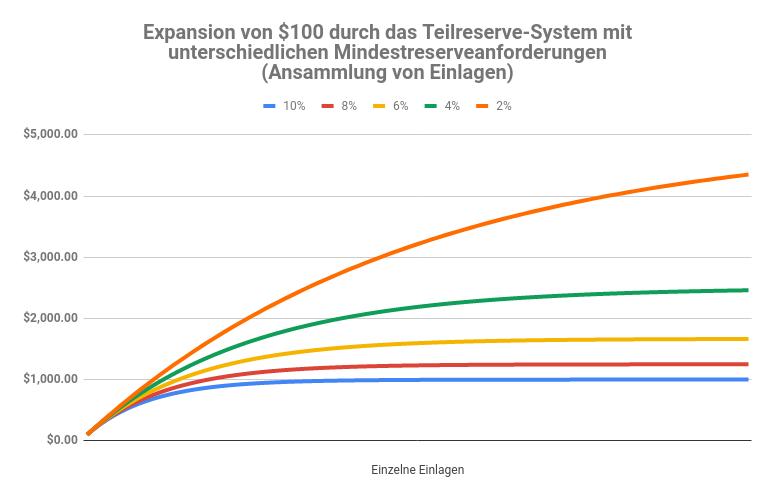
\includegraphics{assets/images/money-multiplier-de.png}
  \caption{Der Geldschöpfungsmultiplikatoreffekt}
  \label{fig:money-multiplier}
\end{figure}

\paragraph{}
Versteh mich nicht falsch: An einer Kreditvergabe ist grundsätzlich nichts
auszusetzen. Auch an Zinsen gibt es nichts auszusetzen. Es gibt nicht mal etwas
an den guten alten Banken auszusetzen, bei denen man sein Vermögen viel sicherer
lagern konnte, als in der Sockenschublade.

Die Zentralbanken sind aber ein anderes Biest. Sie sind halb öffentlich und halb
privat. Sie spielen Gott mit etwas, das jeden betrifft der Teil unserer globalen
Gesellschaft ist, haben kein Gewissen, sind nur an der unmittelbaren Zukunft
interessiert und müssen niemandem Rechenschaft ablegen (siehe
Abbildung~\ref{fig:bsg}).

\begin{figure}
  \centering
  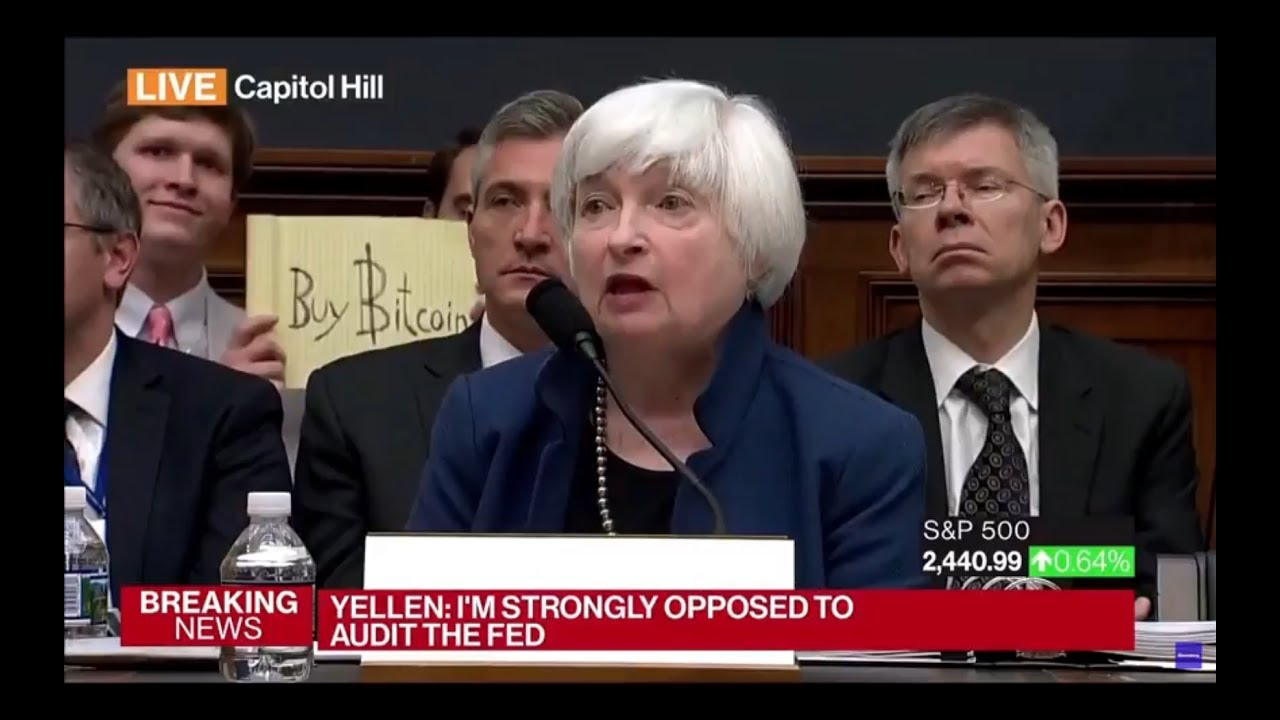
\includegraphics{assets/images/bsg.jpg}
  \caption{Yellen ist entschieden dagegen, die Fed zu prüfen, während Bitcoin
  Sign Guy den Kauf von Bitcoin nachdrücklich befürwortet.}
  \label{fig:bsg}
\end{figure}

Aktuell ist Bitcoin auch noch inflationär, dies wird aber bald aufhören. Das
streng begrenzte Angebot von 21 Millionen Bitcoins wird die Inflation
schließlich vollständig beseitigen. Wir haben jetzt zwei monetäre Welten: eine
inflationäre, in der Geld willkürlich gedruckt wird und die Welt von Bitcoin, in
der das Endangebot fest fixiert und für jeden leicht zu überprüfen ist. Die eine
wird uns durch Gewalt aufgezwungen, die andere kann von jedem der dies wünscht
verwendet werden. Es gibt keine Eintrittsbarrieren und niemanden, den man um
Erlaubnis bitten müsste. Freiwillige Teilnahme. Das ist das Schöne an Bitcoin.

Ich würde argumentieren, dass der Streit zwischen keynesianischen\footnote{Unter
Keynesianismus wird in den Wirtschaftswissenschaften ein auf John Maynard Keynes
zurückgehendes Theoriegebäude verstanden, in dem die gesamtwirtschaftliche
Nachfrage die entscheidende Größe für Produktion und Beschäftigung
ist.~\cite{wiki:keynesian}} und österreichischen\footnote{Als Österreichische
Schule wird eine Gruppe von Theoretikern bezeichnet, die eine bestimmte
heterodoxe Lehrmeinung in der Volkswirtschaftslehre vertreten. Die Schule betont
die Bedeutung der einzelnen Menschen und deren individueller Vorlieben für die
wirtschaftlichen Prozesse (Subjektivismus, Methodologischer
Individualismus).~\cite{wiki:austrian}} Ökonomen nun nicht mehr rein akademisch
ist. Satoshi gelang es ein System für Werttransfer aufzubauen und
damit das solideste/gesündeste Geld zu schaffen, dass es bisher gab. Auf die
eine oder andere Weise werden immer mehr Menschen etwas über den Betrug
erfahren, der uns als Fractional-Reserve-Banking verkauft wird. Falls sie zu
ähnlichen Ergebnissen kommen, wie die Bitcoiner oder Anhänger der
österreichischen Schule der Ökonomie, sind sie frei sich dem ständig wachsenden
Internet des Geldes anzuschließen. Niemand kann sie aufhalten, wenn sie sich
dafür entscheiden.

\paragraph{Bitcoin lehrte mich, dass Fractional-Reserve-Banking purer Wahnsinn ist.}

% ---
%
% #### Down the Rabbit Hole
%
% - [The Creature From Jekyll Island] by G. Edward Griffin
% - [Money Multiplier][money multiplier], [Keynesian Economics][Keynesian], [Austrian School][Austrian] on Wikipedia
%
% [The Creature From Jekyll Island]: https://archive.org/details/pdfy--Pori1NL6fKm2SnY
%
% [joint debate]: https://www.youtube.com/watch?v=hYzX3YZoMrs
% [money multiplier]: https://en.wikipedia.org/wiki/Money_multiplier
% [auditability]: https://i.ytimg.com/vi/ThFGs347MW8/maxresdefault.jpg
% [Keynesian]: https://en.wikipedia.org/wiki/Keynesian_economics
% [Austrian]: https://en.wikipedia.org/wiki/Austrian_School
%
% <!-- Wikipedia -->
% [alice]: https://en.wikipedia.org/wiki/Alice%27s_Adventures_in_Wonderland
% [carroll]: https://en.wikipedia.org/wiki/Lewis_Carroll
